\documentclass[12pt]{article}
\usepackage{fullpage}
\usepackage[utf8]{inputenc}
\usepackage{graphicx}
\usepackage{enumitem}
\usepackage{float}
\usepackage{array}
\usepackage{caption}
\usepackage{subcaption}
\usepackage{array} %to place content in one side of cell in table
\usepackage{datetime}
\usepackage{wrapfig}
\usepackage{amsmath} % to be able to create matrices
\usepackage[headsep=0.5cm,headheight=2cm]{geometry}
\usepackage[parfill]{parskip} %remove the indent (tab) at the beginning of new paragraphs
\usepackage{comment}
\geometry{
a4paper,
total={170mm, 240mm}, %130
left=20mm, %40
top=25mm,
}\usepackage{fancyhdr}

\usepackage[comma,numbers,sort&compress]{natbib}
\bibliographystyle{unsrtnat}
\usepackage[pdfstartview=FitH,
            breaklinks=true,
            bookmarksopen=true,
            bookmarksnumbered=true,
            colorlinks=true,
            urlcolor=blue,
            linkcolor=black,
            citecolor=black,
            ]{hyperref}
\usepackage{pbox}
            
\hypersetup{
    colorlinks=true,
    linkcolor=blue,
    filecolor=blue,      
    urlcolor=magenta,
}

%défini la largeur du trait
\pagestyle{fancy}\renewcommand
\headrulewidth{1pt}
%déclaration du contenu de l'entête
\fancyhead[L]{Zahra Farsijani}
\fancyhead[C]{Medchain}
\fancyhead[R]{Project Report}

\begin{document}

\begin{titlepage}
\center

\includegraphics[width=7.2cm]{Images/EPFL_Logo_SVG.png}\vspace{23pt}\\
\textsc{\Large Laboratory For Data Security (LDS)}\\[0.5cm]

\vspace{25pt}
\hrule
\vspace{0.4cm}
{\Large \bfseries MedChain: A Distributed Authorization and Authentication System for Medical Queries }\\[0.5cm] % Title of your document
\normalsize{Master Semester Project Report}
\vspace{0.4cm}
\hrule 
\vspace{1.5cm}
\begin{minipage}{0.5\textwidth}\large
\begin{flushleft}
\emph{Author:}\\
\textbf{Zahra \textsc{Farsijani}}\\
School of Engineering, Electrical Engineering
\end{flushleft}
\end{minipage}
~
\begin{minipage}{0.4\textwidth}
\begin{flushright} \large
\emph{Professor:} \\
\textbf{Jean-Pierre \textsc{Hubaux}}\\
\emph{Supervisors:} \\
\textbf{Juan \textsc{Troncoso-Pastoriza} }\\
\textbf{David \textsc{Froelicher}}\\
\textbf{Mickaël \textsc{Misbach}}

\end{flushright}
\end{minipage}\\
\vfill
\vspace{5pt}
\vspace{20pt}
{\large \today}\\[12cm]
\vfill
% 	\vspace*{\fill}
% 	\begin{center}
% 		\vspace{0.8cm}
% 		{\LARGE Self-sealing icycle innertubes\\
% 		Assessment of design, manufacturing and marketing feasibility \par}
% 		\vspace{0.7cm}		
% 		{\large Fatemeh Farsijani \\ Pavel Kalinin\\ Raúl Núñez \\ Valentin Perruchoud \\ Rachel Wong Min\par}
% 		\vspace{0.7cm}
% 		\today
% 		\\
% % 		\vspace{0.4cm}
% % 		
\includegraphics[width=6.5cm]{Images/EPFL_Logo_SVG.png}
% 	\end{center}
% 	\vspace*{\fill}
\end{titlepage}		
\pagebreak

%\section*{Abstract}
%\addcontentsline{toc}{section}{\protect\numberline{}Abstract}
\newgeometry{left=3cm,right=3cm}
\begin{abstract}

There is great body of research that depends on use and analysis of clinical and health data as well as sharing them among multiple institutions in some way. This gives rise to some concerns and issues regarding the privacy of data owners due to researchers' access to such sensitive data. A number of software solutions have been developed in order to address this problem and allow privacy-preserving analysis and sharing of sensitive medical data among many institutions such as MedCo \cite{raisaro2018medco}, being the very first operational one. However, when it comes to authentication and authorization of data users, MedCo exhibits some limitations. First, in MedCo, authentication and authorization are central which introduces a single point of failure within the network. Second, each participant in MedCo cluster, runs its own access management process.  

In this project, we propose ``Medchain: a distributed authorization and authentication system for medical queries" that overcomes the drawbacks present in MedCo. Medchain works seamlessly with MedCo and complements its full workflow by handling the access management. Furthermore, Medchain offers auditability as it records all the medical queries from the users in an immutable ledger, i.e., blockchain.

\end{abstract}
\restoregeometry




\pagebreak

\tableofcontents
\pagebreak

\section{Introduction}\label{section1}
\subsection{Problem Definition and Objectives}

In this project, we aim to design and implement a distributed authentication and authorization system for medical queries, called Medchain. We also intend to make this system specifically compatible with the ecosystem of \href{https://medco.epfl.ch/}{MedCo}. MedCo is an existing technology that enables privacy-preserving analysis and sharing of medical data. MedCo already has authentication and authorization mechanisms in place, however, they have some drawbacks which Medchain tries to address. First, in the current implementation of MedCo, both authentication and authorization are centralized. This introduces a single point of failure in the whole ecosystem and has to be avoided. Second, hospitals and medical institutions that participate in MedCo cluster have their own identity providers and run access management protocols individually as these processes can not be done in a federated manner. Our proposed software system, Medchain, offers solutions for such shortcomings. It also puts forward other sought-after properties, such as auditability through the use of blockchains, which is explained in more details later in this report. 


\subsection{Report Outline}
In this report, we first provide some background information needed so that the reader gets a better understanding of the building blocks of Medchain and technologies used in its deployment in Section \ref{section2}. Next, in Section \ref{section3}, design and architecture of Medchain is presented and discussed. In Section \ref{section4}, we give a full descriptions of our solution, its software design and building blocks. Later, in Section \ref{section5}, we show how our software solution meets the requirements and fulfills the original objectives. In Section \ref{section6}, we discuss the future opportunities to improve the solution and, finally, we finish with conclusions in Section \ref{section7}.

\section{Background}\label{section2}
In this section, we provide some background information about the building blocks of our software solution, namely, Medchain and some technologies used in its development. 

\subsection{Cothority}\label{cothority}
The collective authority (cothority) available at \cite{cothority:2019} is a project developed and maintained by DEDIS lab at EPFL. Its goal is to provide various frameworks for development, analysis, and deployment of decentralized and distributed (cryptographic) protocols. In order to be able to access the services provided by cothority, one should run a set of servers that run cothority protocols. Such set of servers is referred to as a \textbf{collective authority} or \textbf{cothority}. Furthermore, every single server in cothority is a cothority node and is called a cothority server or a \textbf{conode}. The code in cothority repository allows the developers to access the services of a cothority and/or run their own conodes. In the following sections, we look at some of the most important building blocks of Cothority as well its services, protocols, and some applications that use it.


 \subsubsection{Conode}\label{background:conode}
As it was mentioned earlier, a \textbf{conode} is server in a cothorit and conodes are linked together to form a cothority. Clients need to run conodes, either locally for local tests or in public mode, in order to access decentralized protocols and services offered by cothority.

To operate a conode, one needs to correctly set up a host and run the conode program. The reader is referred to conode documentation and instructions on how to setup and use it found at \cite{conode:2019}.

\subsection{ByzCoin}\label{background:byzcoin}
ByzCoin in one of the services offered by cothority and there are many cothority applications that use ByzCoin as there building block. ByzCoin is a scalable Byzantine fault tolerant (BFT) consensus algorithm for open decentralized blockchain systems. It uses the skipchain \cite{skipchain:2019} as its underlying data-structure for storing blocks and thus has a distributed ledger holding keys and values. It also implements pre-compiled smart contracts. The \textbf{Omniledger} paper \cite{kokoris2018omniledger} describes the protocol that ByzCoin implements. The reader is referred to \cite{byzcoin:2019} for further details about ByzCoin: how to use it, its building blocks, etc. 

There are various basic data structures used in ByzCoin. Below, we provide a brief overview of the most relevant ones:
\begin{itemize}
    \item{\textbf{Instructions}}: An Instruction is created by a client and it will be executed in ByzCoin. It can be a \texttt{Spawn}, \texttt{Invoke}, or \texttt{Delete} command which results in a \texttt{StateChange} if it is accepted by ByzCoin. The purpose of each command is described below:
    \begin{itemize}
        \item \texttt{Spawn}: create a new instance
        \item \texttt{Invoke}: call a method of an instance such as \texttt{update}
        \item \texttt{Delete}: remove an instance
    \end{itemize}
    
    \item{\textbf{ClientTransaction}}: A \textit{ClientTransaction} holds one or more instructions and is sent by a client to one or more conodes in the roster. 
    \item{\textbf{StateChange}}: Instructions (i.e., ClientTransactions) sent by a client correspond to a contract/object. The execution of these instructions (i.e., the calls to the contracts/objects) results in 0 or more changes in the global state referred to as \textbf{StateChange}. 
    \item{\textbf{Distributed Access Right Controls (Darcs)}}: Darcs offer means to control access rights to the available resources in ByzCoin. Since Darc is one of the most important building blocks of Medchain, we have dedicated a separate section to it. Please refer to Section \ref{background:darc} to learn more about the Darcs. 

\end{itemize}


\subsubsection{Distributed Access Right Controls (Darcs)}\label{background:darc}
Darcs enable us to control access to contracts/objects in ByzCoin and thus can be used for authorization and/or authentication in software systems. Instead of using a password or a public key for authentication, Darcs allow us to implement access control rules that can be \textit{evolved} based on a threshold number of keys. This essentially means that instead of having a static set of rules (e.g., a fixed list of identities that are allowed to access a resource), we can evolve the existing rules any time and thus achieve dynamism in our access right definitions.  

As it was discussed in Section \ref{background:byzcoin}, Darc is one of data structures in ByzCoin. It contains a set of rules that defines what permissions are granted to any identity (i.e., public key). A Darc can be updated by an \textit{evolution} process: the identities that have the evolve permission in the Darc create a signature and sign off the new Darc. There is no limit to the number of evolutions that can be performed and evolutions result in a chain of Darcs, also known as a path. A path can be verified by starting at the oldest Darc (also known as the base Darc), walking down the path and verifying the signature at every step.


Every Darc has a set of rules that are defines as a pair of action/expression. In order for an instruction to be executed on an instance (i.e., an instance of a smart contract stored in the ledger as the global state. Please refer to Section \ref{background:smart_contract} for more details about the smart contracts and instances in ByzCoin), the rules (i.e., the action/expression pair) in the Darc governing the instance have to be met. Every Darc is stored with an \textit{InstanceID} that is equal to the Darc's base ID. Once a Darc is evolved, this InstanceID is overwritten with the new value. Whenever the client sends an instruction for execution, he/she has to also provide the InstanceID of the Darc that governs the corresponding instance that is to be affected by the instruction. Thus, the Darc comes into play and checks if the client has the right to execute the instruction and consequently, approves or rejects the instruction on the instance. This scenario can be summarized into the steps below:

\begin{enumerate}
    \item Client sends the following instruction to ByzCoin (some fields are omitted for clarity):
    \begin{itemize}
        \item \texttt{InstanceID: [32]byte{GenesisDarcID}}
        \item \texttt{Invoke}:
        \begin{itemize}
            \item \texttt{Command: Update}
            \item \texttt{Args: {"Roster": NewRoster}}
        \end{itemize}
        \item \texttt{Signatures: [Sig1]}
    \end{itemize}

    \item ByzCoin finds the Darc instance using the \texttt{InstanceID} provided by the client in the instruction.
    \item ByzCoin creates a \texttt{DarcRequest} using the \texttt{InstanceID} and the \texttt{Args}
    \item ByzCoin checks the Darc found in step 2 and verifies that the request corresponds to the \texttt{invoke:update} rule (i.e., expression) in the Darc instance for the given identity (the client).
\end{enumerate}

Delegation is also possible in Darcs. That is, a Darc can be given \texttt{evolve} permission to evolve other Darcs and thus evolve the path.


\subsection{Smart Contracts and Instances} \label{background:smart_contract}
In Byzcoin, a smart contract is similar to a smart contract in Ethereum. The difference, however, is that in Byzcoin, contracts are pre-compiled and the conode holds the binary of the smart contract. In general, we can say that the smart contract is a collection of methods that provides the client with the API to interact with the skipchain (i.e., the ledger that holds the instances of the contract) through transactions. In other words, contract interprets the methods, namely the instructions, sent by the client for the cothority server (conode). The execution of a client instructions by smart contract results in a change in the shared \textbf{global state}, called a \texttt{StateChange}. In order to commit the transactions onto the ledger, the threshold of agreeing conodes must be reached. A conode can hold various contracts at the same time. Each contract is identified by a string pointing to it called the ``contractID". 

Byzcoin uses coins as the mining reward. As an input, smart contracts receive a list of coins that are available to them. After the contract is run, it needs to give the new list of coins that is available. After all contracts have been run, the leftover coins are given to the leader as a mining reward.

Below, you can find the list of input arguments given to a contract and its output arguments:

\textbf{Input arguments}: 
\begin{itemize}
    \item pointer to database for read-access
    \item Instruction from the client
    \item key/value pairs of coins available
\end{itemize}

\textbf{Output arguments}: 
\begin{itemize}
    \item one StateChange (may be empty)
    \item updated key/value pairs of coins still available
    \item error that will abort the clientTransaction if it is non-zero. If any contract returns non-zero error, the state will not be changed.
\end{itemize}

\subsubsection{Contract Instance Structure}
In ByzCoin, the global state holds the instances of contracts and is split by the Darcs that define the access to control the corresponding instances. Every instruction sent to an instance must resolve the rule in the governing Darc. Every instance is stored with the following information in the global state:

\begin{itemize}
    \item \textbf{InstanceID} is a globally unique identifier of the instance.
    \item \textbf{Version} is the version number of this update to the instance, starting from 0.
    \item \textbf{ContractID} points to the contract that will be called if the instance receives an instruction from the client
    \item \textbf{Data} is interpreted by the contract and can change over time \item \textbf{DarcID} of the Darc that controls access to the instance.
\end{itemize}

\subsubsection{Interaction between Instructions and Instances}
Once a client sends an instruction, he/she indicates the InstanceID to which it corresponds per an instruction argument. ByzCoin tries to first authorize the instruction through the process described in Section \ref{background:darc}, it then uses the InstanceID to look up the responsible contract for the instance and then send the instruction to that contract. 

\subsection{MedCo}\label{background:medco}
MedCo \cite{raisaro2018medco} is the first operational system that enables the exploration and analysis of distributed (sensitive) medical data in a privacy-preserving manner. By using strong collective encryption provided by collective authority \cite{syta2015certificate}, MedCo is able to offer security. MedCo aims to distribute trust among various medical data providers (such as medical institutions) so that their data can be used and queried by external users while privacy is preserved. 

MedCo is built on top of existing and open-source technologies: (i) i2b2 \cite{murphy2010serving} is a clinical research platforms and together with SHRINE \cite{weber2009shared} they enable clinical data exploration; (ii) UnLynx \cite{froelicher2017unlynx} allows distributed and secure data processing in MedCo. 

\section{Design and System Architecture}\label{section3}
\subsection{General Overview} \label{arch:general Overview}
In this section, we will look at the architecture of Medchain system. We first begin by looking at the requirements that our software solution should be able to fulfil. Then, we discuss how the our solution meets its requirements and objectives. 

\subsection{Requirements} \label{arch:requirements}
Medchain aims to offer distributed identity and access management mechanisms for (medical) data sharing systems. However, the main goal of this project is to apply Medchain for a specific medical data system called MedCo described in Section \ref{background:medco}. To achieve this, Medchain has to fulfil the following tasks and requirements:
\begin{enumerate}
    \item Offer its services in a distributed manner 
    \item Offer access management and user authentication 
    \item Authorize users and queries
    \item Enable auditability 
    \item Work seamlessly with MedCo
\end{enumerate}
In the following sections, we study how each of the above-mentioned requirements are fulfilled in Medchain. 

\subsubsection{Distributed Services in Medchain} \label{arch:distributed}
Conodes make the foundation for Medchain. Conodes support distributed protocols and services provided by the \href{https://github.com/dedis/onet/blob/master/README.md}{onet} library (a part of Cothority project developed by DEDIS at EPFL), so does Medchain. 

\subsubsection{Authentication in Medchain}\label{arch:authentication}
The goal of authentication is to verify the identity of the user who wants to access a specific resource such as data. In Medchain, user authentication is delegated to Keycloak \cite{keycloak:2019} which is the identity provider. This means that once Medchain receives a query from a user, we can simply assume that he/she is already authenticated and his/her identity and the user identity is submitted to Medchain as part of the query. We will discuss this in more details in Section \ref{arch:flow}, where the flow of query in Medchain is described comprehensively.

\subsubsection{Authorization in Medchain}\label{arch:authorization}
The goal of authorization is to control the user access to resources (e.g., data) based on his/her access level. In Medchain, we use Darcs (described in Section \ref{background:darc}) to enable user authorization and access management. 


\subsubsection{Auditability of Medchain} \label{arch:audit}
Auditability in Medchain means that there should be a mechanism in place so that the users can track all the queries submitted to Medchain server. Consequently, trace of any data misuse, data abuse, security/privacy breach, etc. can be found and mitigated later. 

In Medchain, we use blockchains to offer auditability. The blockchain framework we used in Medchain is ByzCoin (see Section \ref{background:byzcoin}). Every query sent by the user and its status, whether it is authorized or rejected, is recorded in the immutable ledger. 

\subsection{Medchain High-level View} \label{arch:high-level view}

Figure \ref{fig:medchain_node} shows the full architecture of a Medchain node. Every Medchain node is a conode and it contains three important building blocks. Below you can find more about each of these building blocks and their purpose:
\begin{itemize}
    \item \textbf{Smart contract}: offers user API and distributed access management 
    \item \textbf{Darcs}: manage user's access to resources 
    \item \textbf{Blockchain}: auditability 
\end{itemize}

Additionally, every Medchain node has 1 or more projects in it. A project is an abstract notion that wraps around a specific data resource and restricts access to it. Implementation-wise, every project is, in fact, a Darc that controls the access rights concerning a specific database.

\begin{figure}[ht] 
        \centering 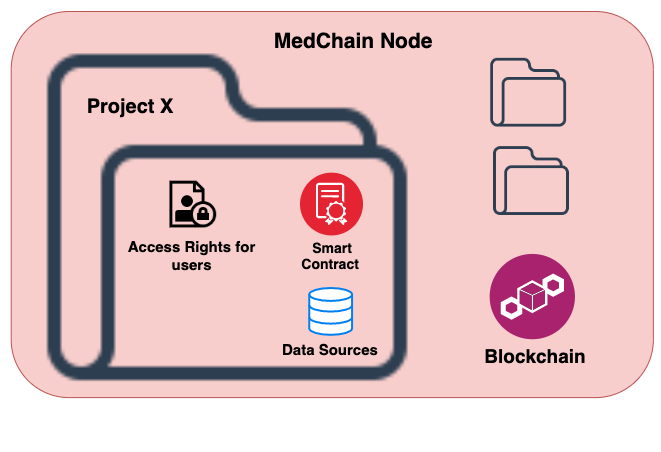
\includegraphics[width=0.7\columnwidth]{Images/medchain_node.png}
        \caption{\label{fig:medchain_node} 
         The structure and building blocks of a Medchain node.
        }
\end{figure}

\subsection{Flow of Queries in Medchain}\label{arch:flow}
Figure \ref{fig:medchain_workflow} illustrates the full architecture of Medchain and its detailed workflow starting from query creation and submission by the client until the query is executed. 

In this figure, there are three hospitals each running their own local Medchain server (conode). Now, focusing only on the user at Hospital 1, we describe the enumerated steps in Figure \ref{fig:medchain_workflow} as following:

\begin{enumerate}
    \item \textbf{User Login}: Client receives the token (i.e., its identity) from Keycloak.
    
    \item \textbf{Query Creation \& Submission}: User spawns a query. The query is submitted to MedCo-connector (i.e., service provider). 
    
    \item \textbf{User Authentication}: MedCo-connector verifies the token (i.e., the identity) of the user. 
    
    \item \textbf{Submission of Query To Medchain}: MedCo-connector sends the query that contains the user’s identity (i.e., part of the token) to Medchain server.
   
    \item \textbf{Query Authorization}: Medchain checks if the query can be executed based on the user identity, what the query is, and the target project according to the Darcs and the associated smart contract. If the query is authorized, Medchain assigns an \texttt{ID} to the query as well as a \texttt{status}. The \texttt{status} of the query is now set to \texttt{Submitted}; the \texttt{ID} of the query contains the name of the project (i.e., data resource) to which it corresponds as well as the token (i.e., the user’s identity) and the actual query (e.g., \texttt{patient\_list}) created by the user. Then, Medchain server creates a transaction using the query, and signs it. 
    
    \item \textbf{Consensus}: The original Medchain node broadcasts the transaction proposal to the rest of the Medchain nodes in cothority network so that it is recorded in the ledger. If a number of Medchain servers in the network are down and/or the responsible entities to accept or reject a query are not present (e.g., a manager at the hospital) at the time of transaction broadcast, the transaction execution is deferred until the threshold number of entities can react to it and either reject or accept it.  

    \item \textbf{Query Execution}: MedCo-connector waits for a signal from Medchain nodes that they have reached consensus over the status of the query (either rejected or authorized) and have committed it to the ledger. If the query is authorized, MedCo-connector executes it, otherwise, the query is disregarded. (In fact, MedCo-connector, i2b2 server, and MedCo-UnLynx all take part in query execution step, however, because the focus here is on Medchain, we overlook the details related to the query execution and only resort to high-level descriptions.) 
    
    \item \textbf{Commit Final Query Status To The Ledger}: MedCo-connector submits the new query status (e.g., “Executed”) to the network of Medchain servers so that its new status is added to the ledger. 
    
\end{enumerate}
 
 
 \begin{figure}[htbp] 
        \centering 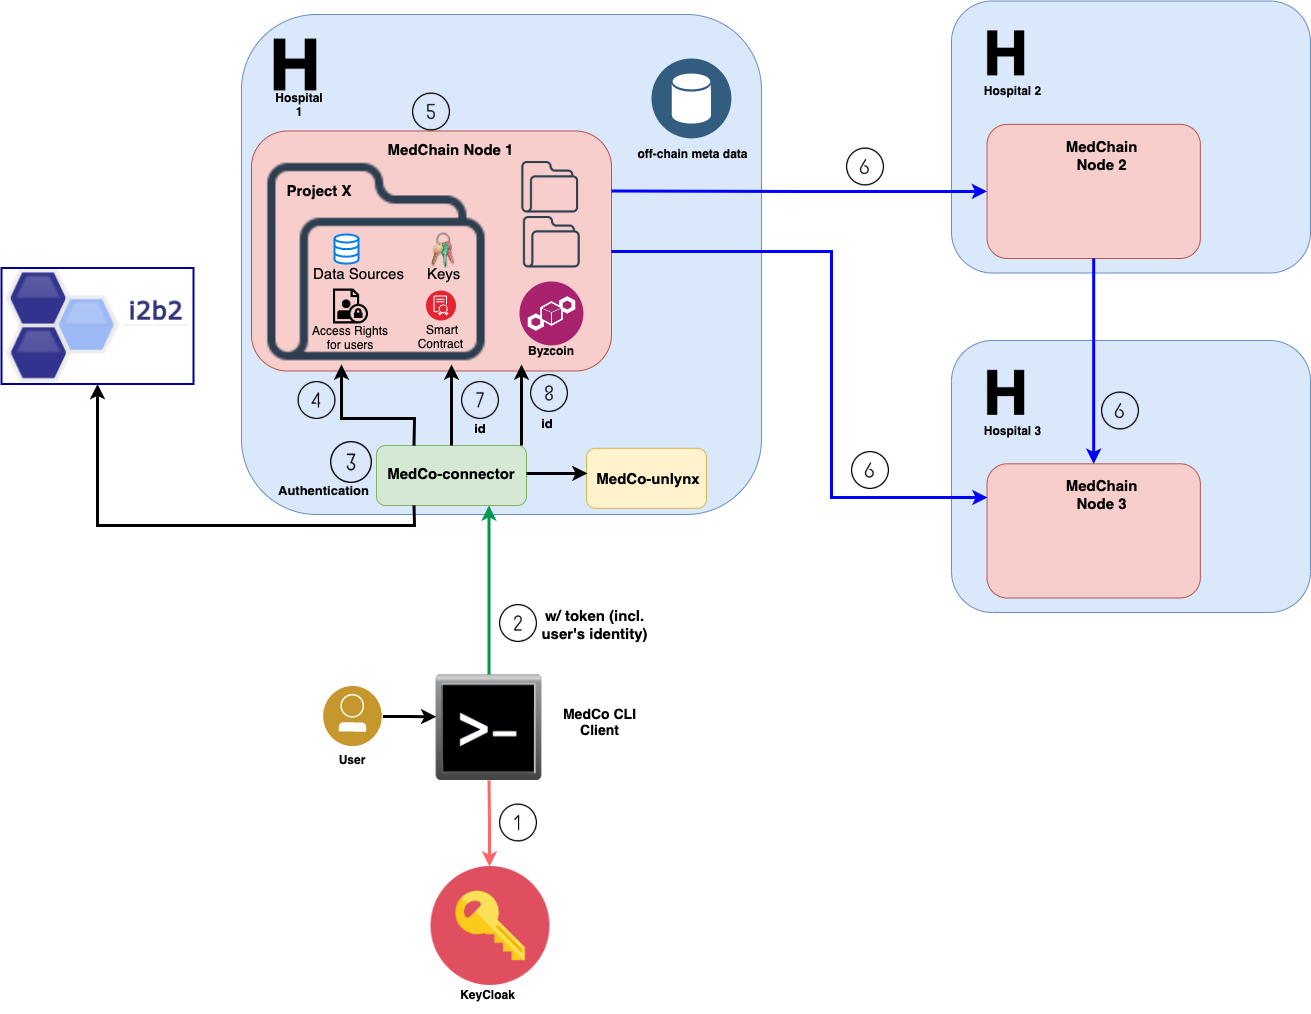
\includegraphics[width=1\columnwidth]{Images/medchain_msg.png}
        \caption{\label{fig:medchain_workflow} 
         Medchain architecture: workflow of queries in Medchain.
        }
\end{figure}


\section{System Implementation}\label{section4}
The full Medchain code, instructions on how to run it and its documentation is available in \href{https://github.com/ldsec/medchain/tree/dev}{Medchain Github repository}. In this section, we aim to provide details about the code structure of the Medchain and not instructions on how to use the code.  

\subsection{Conode}
Every Medchain node is a cothority server, known as a conode. There are several ways to initialize a conode that are described in conode documentation found at \cite{conode:2019}. In this project, we used \href{https://github.com/dedis/cothority/blob/master/conode/README.md#option-1-computer-configuration-setup-with-the-command-line}{configuration setup with the command line} to setup our network of 3 local conodes in an interactive manner. Also, in order to use the conodes we followed the instructions to \href{https://github.com/dedis/cothority/blob/master/conode/README.md#option-1-computer-run-with-the-command-line}{run} them. 

The main point to note here is that once a smart contract is developed and imported into a conode, it is available and can be used by the client. This means that the user does not need to bootstrap the smart contract or install it.  

\subsection{API}
In this section, we provide details about some building blocks of the Medchain Application Programming Interface (API). 

\subsubsection{Smart Contract} \label{impl:smart_contract}
The smart contract provides the user with the API to interact with the skipchain (i.e., the ledger) by adding, updating, or removing the instances of the contract from the ledger. 

We developed the smart contract in Go using the template contract provided in cothority\_template repository called  \href{https://github.com/dedis/cothority_template/tree/master/byzcoin}{ByzCoin example} which is a simple key-value contract, meaning that every instance of the contract that is recorded in the ledger is a key-value store data structure. Medchain smart contract is identified by its name "queryContract". This contract is distinguishable from any other contract used in Medchain deployment such as Darc contracts (see Section \ref{impl:darcs}). The client uses this ID in order to define which contract instance he/she wants to manipulate. The queries submitted to Medchain are recorded in the ledger as instances of queryContract. The structure of these queries is shown below: 

\begin{verbatim}
type Query struct {
	    ID     string //<query_id>:<user_id:databaseX>:<type of query>
	    Status string // "Submitted", "Authorized", or "Rejected"
} 
\end{verbatim}

As it is shown above, the key of a queryContract instance is the ID of the query and the value is its status.  

To serve the purposes of Medchain, we changed some functionalities of the template contract so that it is adapted to Medchain ecosystem. In ByzCoin, the smart contract has to implement three API methods: \texttt{Spawn},\texttt{Invoke}, and \texttt{Delete}. The very first instance of a contract is created by creating a transaction using \texttt{Spawn} as the instruction. By this transaction, the user sets the query ID as the key of the instance and its status as the value. Later, the user can manipulate this instance of the contract by calling an \texttt{Invoke} on it. The \texttt{Invoke} method in queryContract implements two methods itself: \texttt{update} and \texttt{verifystatus}. Using update, the user is able to retrieve a specific contract instance (i.e., query) from the skipchain by its key (i.e., query ID) and update its value (i.e., the status of the query) if it already exists in the skipchain, however, if that is not the case, a new instance of the contract will be spawned using the provided key-value pair. \texttt{verifystatus} method is used by Medchain server itself to retrieve a query from the ledger and verify its status in a similar manner to \texttt{update} method. In Medchain, we decided not to implement the \texttt{Delete} function in contract as we do not want the user to be able to remove a query (i.e., an instance of the contract) from the global state. 

Whenever a contract instance is created (spawned) it is allocated an \texttt{InstanceID} that is based on the ID of the Darc contract governing it (please refer to Section \ref{background:smart_contract} for more details). Later, this instance of the contract is retrievable and authorized by the Darc controlling it using this \texttt{InstanceID}. 

\subsubsection{Deferred Transactions} \label{impl:deferred_tx}
In a real world scenario, it is not always possible for hospitals (running Medchain servers) to approve queries they receive from other Medchain servers instantly, for example, the hospital manager may not be present or the local Medchain server may be down. Thus, the query will be rejected as it will not receive the threshold number of signatures from other Medchain servers in the network it needs so that it is deemed as approved at the time it is created. There should be a mechanism in Medchain to handle this issue. \textbf{Deferred transactions} can be used as a solution for this problem. As the name suggests, deferred transactions allow a transaction to remain idle until it receives the threshold number of signatures it needs to be written in the ledger.  

In order to enable deferred transactions in ByzCoin server, the developer should define a special method in the smart contract, namely, \texttt{VerifyDeferredInstruction}, which is not implemented in a \texttt{BasicContract} (i.e., the basic data structure that all contracts implement by default). In other words, types which embed \texttt{BasicContract} must override this method if they want to support deferred executions (using the \texttt{Deferred contract}). 

\subsubsection{Darcs} \label{impl:darcs}
In ByzCoin, Darcs are used to enable authorization and access management and are, in fact, smart contracts. The only difference between a Darc and a general smart contract is that a Darc supports \texttt{actions} and \texttt{expressions} that are used to define a set of rules in a Darc.

ByzCoin offers some Darcs in its \texttt{darc} library such as \texttt{SecureDarc}, however, the developer can also develop his/her own Darc contract. In Medchain, we use \texttt{SecureContract} and have customized it to meet the requirements of Medchain. 

\texttt{SecureDarc} contract defines access rules for all clients using the Darc data structure. Upon starting a cluster of Medchain servers, a new ByzCoin blockchain and a \texttt{genesis Darc} instance are created. The \texttt{genesis Darc} indicates what instructions need which signatures to be accepted. Below, you can see how the \texttt{genesis Darc} we use in Medchain looks like:

\begin{verbatim}

- Darc:
    -- Description: "genesis darc"
    -- BaseID: darc:<ID_genesis_darc>
    -- PrevID: darc:<ID_darc>
    -- Version: 0
    -- Rules:
        --- invoke:config.update_config - "ed25519:<ID_client>"
        --- spawn:darc - "ed25519:<ID_client>"
        --- invoke:darc.evolve - "ed25519:<ID_client>"
        --- invoke:darc.evolve_unrestricted - "ed25519:<ID_client>"
        --- _sign - "ed25519:3<ID_client>"
        --- spawn:naming - "ed25519:<ID_client>"
        --- spawn:queryContract - "ed25519:<ID_client>"
        --- invoke:queryContract.update - "ed25519:<ID_client>"
        --- invoke:queryContract.verifystatus - "ed25519:<ID_client>"
        --- _name:queryContract - "ed25519:<ID_client>"
        --- invoke:config.view_change - "ed25519:<ID_server> 
            | ed25519:<ID_server> | ed25519:<ID_server>"
    -- Signatures:
    
\end{verbatim}

In the above \texttt{genesis Darc}, we can see the pairs of \texttt{action/expression} that define different rules. For example, \texttt{spawn:queryContract - "ed25519:<ID\_client>"} where \texttt{ID\_client} refers to the ID of the client who is granted the permission for the action \texttt{spawn:queryContract}. Darc expressions are a simple language for defining complex policies. For example, in the rule \texttt{invoke:config.view\_change - "ed25519:<ID\_server> | ed25519:<ID\_server>"}, an "\texttt{or}" expression has been used among the IDs of Medchain cluster servers. 

Now, we create Darcs for different projects (e.g., \texttt{ProjectA} and \texttt{PrjectB}) in Medchain. We assume that each project has 3 clients (i.e., one client per Medchain server). We create new Darcs and define rules (i.e., action/expression pairs) for them. As an example, the Darc for porject A is given below:

\begin{verbatim}
- Darc:
    -- Description: "Project A darc"
    -- BaseID: darc:<ID_darcA>
    -- PrevID: darc:<ID_genesis_darc>
    -- Version: 0
    -- Rules:
        --- _evolve - "ed25519:<ID_client1>" & 
        "ed25519:<ID_client2>" & "ed25519:<ID_client3>"
        --- _sign - "ed25519:<ID_client1>" | 
        "ed25519:<ID_client2>" | "ed25519:<ID_client3>"
        --- spawn:queryContract - "ed25519:<ID_client1>" | 
        "ed25519:<ID_client2>" | "ed25519:<ID_client3>"
        --- invoke:queryContract.update - 
        "ed25519:<ID_client1>" | "ed25519:<ID_client2>" |
        "ed25519:<ID_client3>"
        --- databaseA.patient_list - 
        "ed25519:<ID_client1>" | "ed25519:<ID_client2>" |
        "ed25519:<ID_client3>"
        --- databaseA.count_per_site - 
        "ed25519:<ID_client1>" | "ed25519:<ID_client2>" 
        | "ed25519:<ID_client3>"
        --- databaseA.count_per_site_obfuscated - 
        "ed25519:<ID_client1>" | "ed25519:<ID_client2>" | 
        "ed25519:<ID_client3>"
        --- databaseA.count_per_site_shuffled - 
        "ed25519:<ID_client1>" | "ed25519:<ID_client2>" |
        "ed25519:<ID_client3>"
        --- databaseA.count_per_site_shuffled_obfuscated - 
        "ed25519:<ID_client1>" 
        --- databaseA.count_global - 
        "ed25519:<ID_client1>" 
        --- databaseA.count_global_obfuscated - 
        "ed25519:<ID_client1>" 
    -- Signatures:
\end{verbatim}

In the above Darc for Project A, we have defined rules using different types of actions and expressions. For example, any of the clients is granted permission for action \texttt{databaseA.patient\_list}, however, only client 1 is given permission to query \texttt{count\_global} from database A (i.e., the action \texttt{databaseA.count\_global}). 

Now, let's see how the Darc for Project A can authorize an action. The first step is that the client sends a spawn instruction to Project A Darc contract. Then, the client asks the instance to create a new instance with the \texttt{contractID} of Medchain smart contract, i.e., \texttt{queryContract}, which is different from the ID of the Darc instance itself. The client must be able to authenticate against a \texttt{spawn:queryContract} rule defined in the Project A Darc instance which is indeed the case according to Project A Darc definition above. The transaction that client creates looks like below:

\begin{verbatim}
instr := byzcoin.Instruction{
    InstanceID: byzcoin.NewInstanceID(<Project A Darc ID>),
    Spawn: &byzcoin.Spawn{
    ContractID: "queryContract",
    Args: byzcoin.Arguments{
		    {
		        Name:  < query ID including the action>,
		        Value: []byte("Submitted"), 
		    },
        }  
    },
    SignerCounter: c.nextCtrs(),
}
\end{verbatim}

The new instance spawned will have an instance ID equal to the hash of the Spawn instruction. The client can remember this instance ID in order to invoke methods on it later. In Medchain, we also use \texttt{contract\_name} of ByzCoin. This contract is a singleton contract that is always created in the genesis block. One can only invoke the naming contract to create a mapping from a Darc ID and name tuple to another instance ID. Using this contract, the client does not need to store instance IDs as long as they are named and thus, makes it easier for the client to remember and use the instance IDs of the contracts.

After this step, a queryContract instance spawned by the user (which is in fact the query submitted to Medchain from MedCo) is bound to porject A Darc and is governed by it; thus, the Darc can check for the authorizations of the action the client is trying to take. 

\subsubsection{Client Implementation} \label{impl:client}
To implement a client that can interact with Medchain, we used the default clients  implemented in ByzCoin Client library. The \texttt{Client} is a structure that communicates with the ByzCoin service and interacts with it. 

\subsubsection{Services} \label{impl:services}
In Cothority, a Service is a long term entity that is created when a conode is created. It serves different purposes:
\begin{itemize}
    \item serve the client requests
    \item create and launch protocols in the Overlay network
    \item broadcast to and receive information from services on other conodes within the cothority network. 
\end{itemize}

In Medchain, we mainly used two services: ByzCoin and Onet service. These services handle client-server communications and enable the user to interact with the conodes. We define Medchain API using these services and later implement the CLI-program on top of this API (see Section \ref{impl:cli}). Table \ref{tbl:med_api_calls} shows some of the most important API calls defined in Medchain as well as resources they take and their responses.

\begin{table}[ht]
\centering
\caption{Some of Medchain API calls}
\label{tbl:med_api_calls}
\begin{tabular}{|l|l|l|l|}
\hline
\textbf{Name of Method} & \textbf{Description} & \textbf{Resources} & \textbf{Response}\\
\hline
\textbf{CreateQueryAndWait}    &  Spawn a query & \pbox{20cm}{ User ID, \\ Query definition, \\ Query ID }  & OK?\\
\hline
\textbf{UpdateQueryStatus} & Update the status of a query & Query ID  &  OK? \\
\hline
\textbf{VerifyQueryStatus} & Verify the status of a query & Query ID  &  OK? \\
\hline
 
\end{tabular}
\end{table}

To be able to use the services, we need to register them with the default \href{https://github.com/dedis/cothority/blob/master/suite.go}{Cothority suite}. We use the services to define the API and interact with conodes and contracts.


\subsection{App and Command-Line Interface (CLI)}\label{impl:cli}
An application, in the context of Onet, is a CLI-program that interacts with one or more conodes through the use of the API defined by one or more services. 

We implemented the CLI for Medchain using \href{https://github.com/dedis/cothority/tree/master/byzcoin/bcadmin}{bcadmin} library. The CLI allows the user to start a new ByzCoin blockchain, register new users, initialize and manage pre-developed Darcs, interact with the smart contract, etc. through the command-line. The code for this CLI-app is found in \textit{app/} directory of Medchain repository. 

%\subsection{Docker-based Implementation}\label{impl:docker}
%TODO

\section{System Evaluation}\label{section5}
\subsection{Fulfilment of Requirements}

\subsection{Limitations}


\section{Future Work}\label{section6}
In this section, we would like to offer some opportunities for further improving our implemented software solution and the results of this project. 

\subsection{Integration with MedCo}
One of the main purposes and requirements of Medchain is to make it work seamlessly with data service providers, specifically MedCo. However, given that this requirement was not fulfilled in the scope of this project, the full integration of Medchain into MedCo is expected to be done in future versions of Medchain.  

\subsection{Use of Deferred Transactions}
Although we were able to implement deferred transactions in Medchain, we have not been able to test their functionality in this project and we are not sure if they function properly. Therefore, it is expected that in the future this functionality will be tested and debugged if necessary. 
%\subsection{Improvements}

\section{Conclusion}\label{section7}
In this project, we designed and implemented a distributed authorization and access management system for medical queries called Medchain. Medchain is written in Go and is based on an existing distributed framework called Cothority and runs on conodes. It enables distributed access management through the use of smart contracts (Darcs) and offers auditability through the use of permissioned blockchains for recording all the queries it receives over its lifetime. Medchain is mainly designed to work seamlessly with MedCo and overcome MedCo's authorization limitations.

Medchain supports a CLI interface that enables the user to interact with the cluster of servers through the command-line. In future versions of Medchain, we aim to integrate it with MedCo ecosystem and have it work as part of the whole MedCo workflow. We will also improve its front-end and the user interface.    




%\newpage

%\section{Appendix}\label{section11}
%\input{11Appendix.tex}


\pagebreak
%%%%%%%%%%%%%%%% Bibliography %%%%%%%%%%%%%%%%
\addtocontents{toc}{\vspace{.5\baselineskip}}
\addcontentsline{toc}{section}{\protect\numberline{}{References}}
\bibliography{bibliography}

\end{document}